%! Author = danielmendes
%! Date = 05.01.25
\chapter{Tools}\label{sec:tools}

\section{Auswahl der Tools}\label{sec:auswahl-der-tools}

Die Grundlage für diese Bachelorarbeit ist das Verhalten der MySQL – Datenbank \cite{sysbench_mysql} in Bezug auf die unterschiedlichen Aspekte, die im Rahmen dieser Arbeit behandelt werden.
Der folgende Abschnitt beschäftigt sich mit Umsetzung, um dieses Verhalten messbar und veranschaulich mithilfe von Grafiken zu machen.
Damit wir die Kennzahlen für bestimmte Abfragen an die MySQL – Datenbank bestimmen können, brauchen wir ein zentrales Tool.
Dieses Tool ist dafür verantwortlich ist die Benchmark - Tests durchzuführen.

Meine Entscheidung ist dabei schlussendlich auf Sysbench \cite{sysbench_repo} gefallen.
Sysbench ist ein Open-Source-Tool, das ein skriptfähiges, multi-threaded Benchmark-Tool ist, das auf LuaJIT basiert.
Es wird hauptsächlich für Datenbankbenchmarks verwendet, kann jedoch auch dazu eingesetzt werden, beliebig komplexe Arbeitslasten zu erstellen, die keinen Datenbankserver erfordern.
Sysbench analysiert dabei Metriken, wie unter anderem Transaktionen pro Sekunde, Latenz und Anzahl an Threads.
Dabei kann man genauer spezifizieren, wie oft diese Metriken geloggt werden sollen.
Sysbench ist dabei nicht auf ein einziges Datenbanksystem eingeschränkt, sondern man kann sich zwischen vielen unterschiedlichen Systemen entscheiden.

Im Zuge der Wahl des Benchmark – Tools habe ich auch andere Benchmarking-Tools betrachtet, wie beispielsweise Benchbase \cite{DifallahPCC13} oder mybench \cite{mybench_repo}.
Im Vergleich zu diesen Tools bietet Sysbench jedoch die Vorteile der höheren Skriptfähigkeit und Flexibilität.
Damit ist gemeint, dass bei Sysbench das erste Projekt mit mehr Aufwand verbunden ist als bei den Alternativen.
Wenn man aber ein Projekt erstmal erstellt hat, dann ist es sehr individuell und man kann schnelle Änderungen hervornehmen.
In dem Kapitel (TODO (Daniel): Kapitel mit Join Typ) betrachten wir ein beispielhaftes Projekt mit Sysbench, bei dem der Einfluss von unterschiedlichen Datentypen als Join-Operator zwischen zwei Tabellen verglichen wird.
Wenn wir später die Performance von unterschiedliche Index-Typen betrachten, dann müssen wir nur an wenigen Stellen Veränderungen durchführen, die in dem Kapitel genauer besprochen werden.

Ein weiterer Vorteil von Sysbench ist, dass es als de facto Standard im Bereich der Datenbankbenchmarks angesehen wird \cite{mybench_comparison}.
Durch diese Position gibt es viele aktive Nutzer und dadurch bedingt viele verfügbaren Ressourcen.
Vorteile der anderen Tools sind jedoch die weniger präzise Steuerung der Ergebnisraten und der Transaktionen von Sysbench.
Zudem ist Sysbench auf das Minimale beschränkt, was den Output angeht, da es, wie schon erwähnt, nur eine Reihe von Log-Dateien gibt und
die Visualisierung der Ergebnisse muss vom Benutzer selbst mithilfe von anderen Tools umgesetzt werden.
Anders sieht dies bei dem Tool mybench aus, da es dort die Möglichkeit gibt in Echtzeit umfassende Abbildungen zu betrachten \cite{mybench_user_interface}.
Obwohl dieses Feature sehr hilfreich ist, bin ich nach Abwägung der Vor- und Nachteile zu dem Entschluss gekommen, dass die einfachere Bedienung und die Tatsache,
dass Sysbench der de facto Standard ist, für mich überwiegen, weshalb ich mich für Sysbench entschieden habe.

Nichtsdestotrotz kann nicht komplett auf Graphen verzichtet werden, da Entwicklungen im Laufe einer Zeitmessung in einem Kurvenverlauf deutlich besser zu erkennen sind als in einer Log - Datei.
Anhand der reinen Zahlen lassen sich unter Umständen Trends von zwei oder etwas mehr unterschiedliche Messungen erkennen, aber besonders wiederkehrende Trends werden aus der schriftlichen Form nicht schnell ersichtbar.
Ganz anders sieht dies bei Graphen mit einer Zeitachse aus.
Dort werden sofort Trends ersichtlich und auch der Vergleich zwischen den unterschiedlichen Messungen erfolgt deutlich besser.

Um die Kennzahlen, die mithilfe von Sysbench ermittelt worden sind, in eine grafische Darstellung umzuwandeln, gibt es unterschiedliche Tools, die wiederum einige Vor - und Nachteile mit sich bringen.
Das erste mögliche Tool stellt Gnuplot \cite{gnuplot} dar, mit dem sich CSV – Dateien sehr gut darstellen lassen.
Wenn man aber nur bestimmte Spalten aus der Tabelle darstellen lassen, dann kommt man schnell an seine Grenzen.
Deshalb habe ich mich für eine anpassungsfähigere Alternative entschieden, denn die Transformationen und die grafische Darstellung wird mithilfe eines Python Scripts umgesetzt.
Für die grafische Darstellung sind dabei die Libraries pandas \cite{reback2020pandas} und matplotlib.pyplot \cite{hunter_2007} verantwortlich.

\section{Einführung in die Tools}\label{sec:einfuhrung-in-die-tools}

Als allererstes muss der MySQL – Server gestartet sein.
Dabei ist es egal, ob dies lokal auf dem Rechner oder über einen Docker in eines GitHub CI/CD-Workflows erfolgt.
Das Wichtigste dabei ist es, dass man sich die Zugangsdaten, bestehend aus User - und Passwortdaten, zwischen speichert, da diese gebraucht werden, um den Benchmarktest mit Sysbench zu starten.
Nachdem das RDBMS gestartet worden ist, muss zudem eine Datenbank erstellt werden.
Dies könnte unter anderem so aussehen:

\lstinputlisting[
    language=sql,
    caption=Create Database,
    label={lst:create_db},
    style=custom_daniel,
]{Scripts/Benchmark/database.sql}

Nach der erfolgreichen Erstellung der Datenbank muss das Tool Sysbench installiert werden.
Um sich mit dem Tool Sysbench vertraut zu machen, gehen wir die verschiedenen Argumente, die beim Aufruf mitgegeben können oder müssen, durch.
Darunter gehören:

\begin{itemize}
    \item \texttt{--db-driver}: Gibt den Treiber für die Datenbank an, die Sysbench verwenden soll. In diesem Fall \texttt{mysql}, um die MySQL-Datenbank zu testen.
    \item \texttt{--mysql-host}: Der Hostname oder die IP-Adresse des MySQL-Servers. Standardmäßig wird \texttt{localhost} verwendet, wenn nichts angegeben wird.
    \item \texttt{--mysql-user}: Der Benutzername, mit dem Sysbench auf die MySQL-Datenbank zugreift.
    \item \texttt{--mysql-password}: Das Passwort für den MySQL-Benutzer. Falls der Benutzer kein Passwort hat oder der Zugriff über eine andere Authentifizierungsmethode erfolgt, kann dieses Argument weggelassen werden.
    \item \texttt{--mysql-db}: Der Name der MySQL-Datenbank, auf die zugegriffen wird. In diesem Beispiel \texttt{sbtest}.
    \item \texttt{--time}: Gibt die Laufzeit des Benchmarks in Sekunden an und muss immer mit angegeben werden.
    \item \texttt{--report-interval}: Gibt das Intervall in Sekunden an, in dem Zwischenergebnisse während des Tests ausgegeben werden.
    Sofern \texttt{--report-interval} nicht gesetzt wird, werden die Ergebnisse nur am Ende des Tests angezeigt.
    \item \texttt{--tables}: Die Anzahl der Tabellen, die für den Test erstellt werden sollen. Standardmäßig wird nur eine Tabelle erstellt.
    \item \texttt{--table-size}: Die Anzahl der Datensätze (Zeilen) pro Tabelle. Muss auch nicht zwingend angegebend werden.
\end{itemize}

Neben den sieben aufgelisteten Argumenten gibt es zwei weitere wichtige Optionen:
\begin{enumerate}
    \item Wie im Abschnitt~\ref{sec:einfuhrung}(TODO(Daniel): Abschnitt einfügen) erwähnt, kann ein Lua-Skript angegeben werden, um eigene
    Tabellen zu erstellen, Beispieldaten einzufügen und bestimmte Abfragen durchzuführen.
    Dazu muss am Ende der Sysbench-Befehlszeile lediglich der Pfad zur Lua-Datei hinzugefügt werden.
    Ein erklärendes Beispiel dazu folgt weiter unten in diesem Abschnitt.
    \item Die Methode, den Sysbench ausführen soll, muss ebenfalls spezifiziert werden.
    Auch dieser wird am Ende der Sysbench-Befehlszeile angehängt.
\end{enumerate}

Zunächst schauen wir ein kurzes Demo-Beispiel, denn es gibt die Möglichkeit die Datenbank
auf Performance zu testen, ohne selbst eigene SQL-Befehle zu schreiben. Dafür gibt es vordefinierte Testtypen von Sysbench.
Auf diese Weise kann man schnell die Korrektheit der Einrichtung des Tools überprüfen, bevor man Lua-Scripts
für die eigenen Bedürfnisse schreibt.

Man kann unter anderen zwischen diesen Testtypen wählen:
\begin{itemize}
    \item \textbf{oltp\_insert}: Prüft die Fähigkeit der Datenbank, Daten schnell und effizient einzufügen und
    simuliert eine Umgebung, in der viele Schreiboperationen ausgeführt werden.
    \item \textbf{oltp\_read\_only}: Fokussiert sich auf die Performance bei Leseoperationen und
    eignet sich, um die Leistung bei einer rein lesenden Arbeitslast zu testen.
    \item \textbf{oltp\_read\_write}: Simuliert eine realistische Arbeitslast, bei der sowohl Lese- als
    auch Schreiboperationen gleichzeitig durchgeführt werden.
\end{itemize}

Des Weiteren gibt es auch unterschiedliche Methoden, die mit den Testtypen kombiniert werden können.

\begin{itemize}
    \item \textbf{prepare}: Bereitet die Datenbank für den Test vor, u.a. das Erstellen von benötigten Tabellen.
    \item \textbf{run}: Ist die Ausführungsphase des Tests. Je nach Testtyp führt diese Methode die spezifizierten Operationen aus,
    wie etwa das Einfügen von Daten (oltp\_insert), das Abfragen von Daten (oltp\_read\_only) oder beides (oltp\_read\_only).
    Dabei wird die Performance der Datenbank unter der angegebenen Arbeitslast gemessen.
    \item \textbf{cleanup}: Diese Methode sorgt dafür, dass nach Abschluss des Tests alle Testdaten entfernt werden.
    Sie stellt die Datenbank in ihren ursprünglichen Zustand zurück und stellt sicher,
    dass keine Testdaten zurückbleiben, die eine mögliche produktive Umgebung beeinträchtigen könnten.
\end{itemize}

Für das Demo-Beispiel wählen wir den Testtypen \textbf{oltp\_read\_write} und allen Methoden aus.
Für die Methode run würde unsere Query so aussehen, wobei \texttt{YOUR\_USER} und \texttt{YOUR\_PASSWORD}
entsprechend ersetzt werden müssten:

\begin{lstlisting}[style=custom_daniel,label={lst:sysbenchrun}]
sysbench oltp_read_write \
  --db-driver=mysql \
  --mysql-user=YOUR_USER \
  --mysql-password=YOUR_PASSWORD \
  --mysql-db="sbtest" \
  --time=10 \
  --report-interval=1 \
  run
\end{lstlisting}

Wenn man nur diese Query ausführt, fällt er auf, dass die Query scheitert.
Die Fehlermeldung lautet dabei wie folgt:
\begin{lstlisting}[style=custom_daniel,label={lst:error}]
FATAL: MySQL error: 1146 "Table 'sbtest.sbtest1' doesn't exist"
\end{lstlisting}
Der entstandene Fehler wird offensichtlich dadurch verursacht, dass die Tabelle nicht erstellt worden ist.
Die Lösung für dieses Problem ist die Ausführung der \texttt{prepare} - Methode vor der \texttt{oltp\_read\_write} - Methode.
Damit sich die Datenbank wieder im Anfangszustand befindet noch anschließend an die \texttt{oltp\_read\_write} - Methode noch die \texttt{cleanup} aufrufen werden.
Um sich die manuelle Ausführung dieser drei Befehl in der korrekten Reihenfolge zu sparen, bietet es sich an, ein Shell-Script zu schreiben, indem zuerst die Methoden nacheinander aufgerufen werden.

\lstinputlisting[
    language=bash,
    caption=Process of Sysbench commands,
    label={lst:sysbench_monitor},
    style=custom_daniel,
]{Scripts/Benchmark/process_sysbench.sh}

Die Ergebnisse werden nun der Log-Datei (unter output/sysbench.log) gespeichert.
Damit fehlt uns nur noch die Erstellung der Graphen.
Um uns diese Erstellung zu vereinfachen, bietet es sich an, dass aus der Log - Datei die entsprechende Kennzahlen extrahiert und die Werte mit korrekten Spaltenüberschriften in einer CSV-Datei speichert.
Dies geht mit dem Shell - Kommando \texttt{grep}:

\lstinputlisting[
    language=bash,
    caption=Extraction from log to CSV,
    label={lst:extraction_csv},
    style=custom_daniel,
]{Scripts/Benchmark/extraction_csv.sh}

Als letzten Schritt gibt es die Erstellung der Graphen mithilfe von der Tools Gnuplot oder der Python - Library Pandas.
Die kompletten Scripts \texttt{plot\_sysbench.gp} und \texttt{generatePlot.py} befinden sich am Ende dieser Bachelorarbeit.
Das Python-Script, das zuständig ist für die Graphgenerierung muss als Argument zum einen
die CSV-Datei übermittelt bekommen und zum anderen kann es nur eine bestimmte Auswahl an
Messwerten übergeben, damit nur für diese die Graphen erzeugt werden.

\lstinputlisting[
    language=bash,
    caption=Generation of graphs,
    label={lst:graph_generation},
    style=custom_daniel,
]{Scripts/Benchmark/graph_generation.sh}

\begin{figure}[!ht]
    \centering
    \begin{subfigure}[t]{0.48\textwidth}
        \centering
        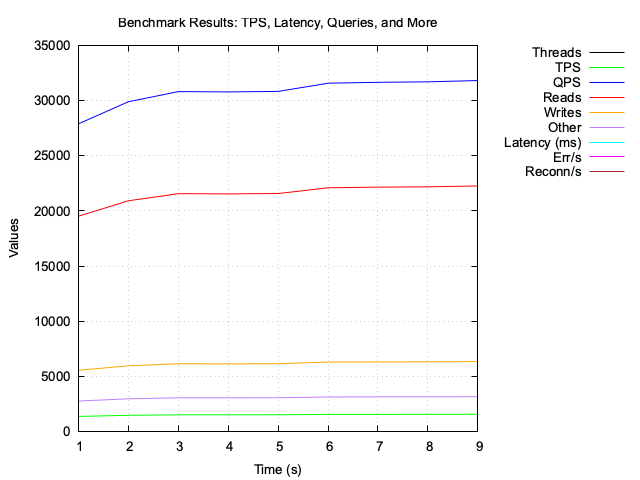
\includegraphics[width=\textwidth]{PNGs/Demo/sysbench_output}
        \label{demo-gnuplot}
    \end{subfigure}
    \hfill
    \begin{subfigure}[t]{0.48\textwidth}
        \centering
        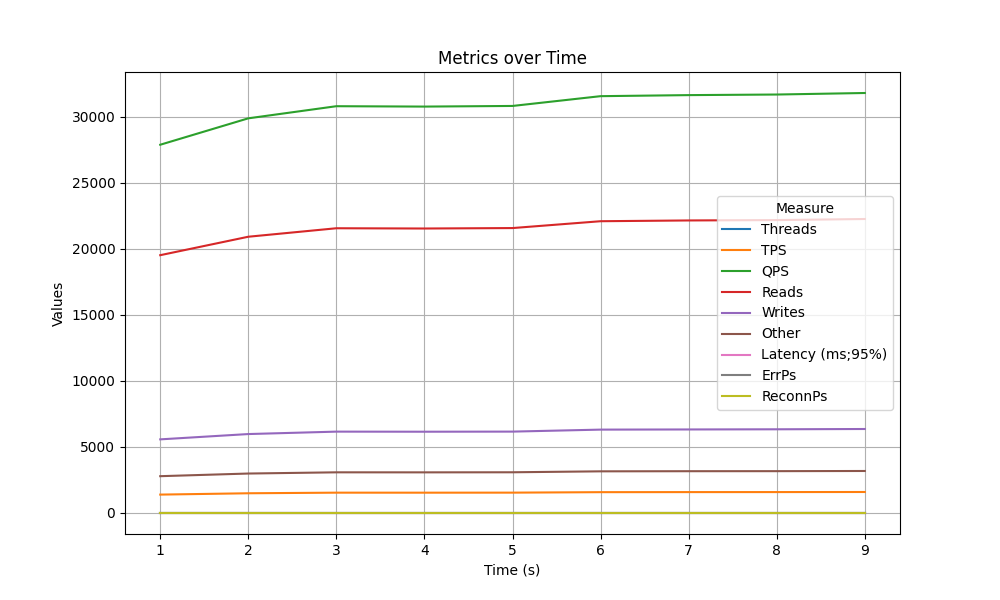
\includegraphics[width=\textwidth]{PNGs/Demo/Summary}
        \label{demo-pandas}
    \end{subfigure}
    \caption[Demo-Graphs: Gnuplot vs. Pandas]{Die Grafik zeigt die erstellten Graphen mit Gnuplot (links) und Pandas (rechts)}
    \label{fig:demo-graph-generation}
\end{figure}


\begin{itemize}
    \item \textbf{Threads}: Die Anzahl der gleichzeitig verwendeten Threads.
    Mehr erhöhen die Parallelität, jedoch zu viele können zur Überlastung des Systems führen.
    \item \textbf{TPS (Transactions Per Second)}: Die Anzahl der Transaktionen pro Sekunde.
    Ein höherer Wert deutet auf eine bessere Datenbankleistung hin.
    \item \textbf{QPS (Queries Per Second)}: Die Anzahl der Abfragen pro Sekunde.
    Ein höherer Wert ist besser und zeigt die Effizienz bei der Verarbeitung von Abfragen.
    \item \textbf{Reads}: Die Anzahl der Leseoperationen.
    \item \textbf{Writes}: Die Anzahl der Schreiboperationen.
    \item \textbf{Other}: Bezieht sich auf andere Arten von Operationen, die weder als Reads noch als Writes kategorisiert werden.
    \item \textbf{Latency (ms; 95\%)}: Die durchschnittliche Zeit in Millisekunden, die benötigt wird, um Anfragen zu bearbeiten, wobei der Wert im 95. Perzentil betrachtet wird.
    Niedrigere Werte sind besser, da sie auf schnellere Reaktionszeiten hinweisen.
    \item \textbf{ErrPs (Errors Per Second)}: Die Anzahl der Fehler pro Sekunde.
    Ein niedriger Wert weist auf höhere Stabilität und Zuverlässigkeit des Systems hin.
    \item \textbf{ReconnPs (Reconnects Per Second)}: Die Anzahl der Wiederverbindungen pro Sekunde.
    Häufige Wiederverbindungen können auch auf Stabilitätsprobleme hindeuten.
\end{itemize}


% TODO (Daniel) missing: how the script and results exactly are fpr Join_Type and explain the measures underneath